%=============================================================================
% Thesis Template in LaTex
%
% File:  02-Grundlagen und Theorie -- Grundlagen
% Author(s): Cyrano Golliez <golliezc@student.ethz.ch>>
%            
%
% Creation:  27 Jan 2014
% Time-stamp: <Tue 2013-08-13 20:14 juergen>
%
% Copyright (c) 2014 Infrastructure Management Group (IMG)
%               http://ibi.ethz.ch
%
% More information on LaTeX: http://www.latex-project.org/
%=============================================================================

\chapter{Grundlagen und Theorie}
\label{chap:Grundlage}

Diese theoretischen Grundlagen sind anhand der Unterrichtsmaterialien des Kurses System Engineering HS 2019 von Prof. Dr. Bryan T. Adey, Dr. Craig Richmond und Dr. Clemens Kielhauser, erarbeitet worden. Der Grossteil der Informationen beziehe ich aus dem Skript zum Kurs. Zur weiteren Vertiefung habe ich die von Dr. Claudio Martani zur Verfügung gestellten Materialien zur Anwendung der \textit{Real Option Methodology} konsultiert.  

\section{Problemlösungsprozess}
\label{sec:Problemprozess}

Der Problemlösungsprozess ist eine universell einsetzbare Methodik zur Bestimmung der optimalen Lösung eines Problems. Anhand dieses systematischen Prozesses kann gewährleistet werden, dass bei der Optimierung eines Systems alle Aspekte zum richtigen Zeitpunkt berücksichtigt werden. So wird sichergestellt, dass die Bedürfnisse der vom betrachteten System abhängigen Personen befriedigt werden und die Funktionalität der erarbeiteten Lösungsvarianten gewährleistet ist. (\cite{Adey2019}) 

\begin{figure}[h!]
	\centering
	\includegraphics[width=\textwidth]{figures/f-02-01-Problemlösungsprozess}
	\caption[Schritte des Problemlösungsprozesses]{Schritte des Problemlösungsprozesses aus (\cite{Adey2019})}
	\label{img:Problemlösung}
\end{figure}

Nachfolgend werden die in Abbildung \ref{img:Problemlösung} dargestellten Schritte des Problemlösungsprozesse anhand des Skript des Kurses System Engineering, kurz erläutert. 

\paragraph{Anstoss} Im ersten Schritt werden die Grenzen und wirkenden Mechanismen des Problemfeldes identifiziert, ein allgemeines Verständnis für das Problem entwickelt und überprüft ob das richtige Problem angegangen wird. Dies erfolgt anhand der Differenzierung zwischen Wunsch und Wirklichkeit und der Bestimmung des Umfangs der Bedürfnisse nach einer geänderten Situation.

\paragraph{Situationsanalyse} Der Zweck einer Situationsanalyse ist einerseits, die Basis für die Konkretisierung der Ziele zu schaffen und andererseits das Problem und die Notwendigkeit einer Intervention zu identifizieren. Weiter sollen die Zusammenhänge zwischen den Ursachen und dem Problem untersucht werden. Dies erfolgt mit der strukturierten Abgrenzung des Problemfeldes und einer detaillierten Darstellung der Ausgangssituation sowie der Aufgabenstellung. Anhand der Begrenzung des Problemfeldes auf den Bereich des Systems, der im Rahmen der Problemlösung optimiert werden soll, und der geschaffenen Informationsbasis können die nachfolgenden Schritte durchgeführt werden. Wichtige in diesem Schritt, für die erfolgreiche Optimierung einer Problemstellung ist die Bestimmung der Diskrepanz zwischen Wunsch und Wirklichkeit.

\paragraph{Formulierung der Ziele und Rahmenbedingungen} In diesem Schritt werden alle Ziele, Wünsche und Absichten der beteiligten Personen zusammengetragen und ausführlich beschrieben, was und in welchem Umfang erreicht werden soll. Diese Beschreibung soll möglichst vollständig, realistisch und objektiv sowie präzise und verständlich formuliert sein. Ausserdem muss bei der Formulierung darauf geachtet werden, dass die Erfüllung der Ziele feststellbar und das Setzen von Prioritäten möglich ist. 

\paragraph{Generierung von möglichen Lösungen} Unter diesem Stichpunkt werden mögliche Lösungen für die Erfüllung der Ziele generiert. In einem ersten Schritt wird das neu zu gestaltende Objekt genauer untersucht und anschliessend werden erste Lösungsideen entworfen. In einem zweiten Schritt werden alle als untauglich erachteten Lösungsideen aussortiert und die verbleibenden möglichen Lösungsvarianten ausgearbeitet. 
Das Konkretisierungsniveau der Varianten soll der Planungsphase entsprechen, in der sich das Projekt befindet. Dieser Schritt erfordert viel Kreativität, da mit einem vertretbaren Aufwand eine Visualisierung und Beschreibung der Varianten erschaffen werden muss, mit der ein neutraler Betrachter das angewandte Konzept, mit dem das Problem gelöst werden soll, erkennen kann.

\paragraph{Analyse von möglichen Lösungen} In dieser Phase des Problemlösungsprozess, werden die Lösungsvarianten auf allfällige Schwachstellen überprüft. Dieser Schritt ist insofern sehr wichtig, da er aufzeigt, ob ein Lösungskonzept den gestellten Anforderungen entspricht. Dies erfolgt durch die Überprüfung der Varianten in Hinblick auf die Erfüllung aller Rahmenbedingungen und Ziele. 

\paragraph{Bewertung von möglichen Lösungen} Die Bewertung der Lösungen dient dazu, die am besten geeignete Variante zu ermitteln. Durch das systematische Vergleichen der Lösungsvarianten, wird eine objektive Entscheidungsfindung ermöglicht. Eine solche Entscheidungsfindung wird mithilfe von Entscheidungsbäumen dargestellt. 

\paragraph{Durchführung} Die Durchführung schliesst den Problemlösungsprozess ab und beinhaltet die Ausführung der Variante, die im Bewertungsprozess als die Beste identifiziert wurde. Die Durchführung ist abhängig von der Phase, in der sich das Projekt befindet. Dies kann z.B. der Start einer Detailstudie (nach der Vorstudie) oder den Bau der Lösungsvariante (nach der Detailstudie), bedeuten.

\section{Interessensgruppen}
\label{sec:Inter.gruppen}

Als Interessensgruppen werden die Einzelpersonen, Gruppen oder Organisationen definiert, die von einer Veränderung der öffentlichen Infrastruktur betroffen sind. Die Interessensgruppen können in zwei Stufen unterteilt werden. Die erste Stufe umfasst die Interessensgruppen, deren Netto-Nutzen maximiert werden soll. Dies beinhaltet zum einen die Besitzer der Infrastruktur und die Nutzer sowie die direkt und indirekt betroffene Öffentlichkeit. Im Falle der zwei letztgenannten Interessensgruppen ist die Zuteilung von der Zeit abhängig. So kann eine Person beim Befahren der Infrastruktur ein Nutzer und zuhause in seiner an die Infrastruktur angrenzenden Liegenschaft, Teil der direkt betroffenen Öffentlichkeit sein. Die zweite Stufe umfasst die Interessensgruppen, die von der Maximierung des Netto-Nutzens der Interessensgruppen der ersten Stufe beeinflusst werden. Diese werden, sofern sie nicht Teil einer Interessensgruppe der ersten Stufe sind, nicht weiter berücksichtigt oder nur falls dies explizit gefordert wird. (\cite{Adeyetall2019})

\section{Zielfunktion}
\label{sec:Zielf}

Um die optimale Lösung zu bestimmen, können im Problemlösungsprozess mathematische Modelle verwendet werden. Viele der verwendeten Modelle zur Optimierung von Problemen haben eine einheitliche Aufbau aus einer Zielfunktion, die es zu maximieren oder minimieren gilt, sowie aus Nebenbedingungen, die die Grenzen der Varianten definieren. Die Zielfunktion sowie die Nebenbedingungen können linear oder nichtlinear sein.
Bei der Analyse von Varianten ist ein sogenanntes Lineares Programm (LP) mit einer linearen Zielfunktion und lineare Nebenbedingungen äusserst hilfreich, das dieses mit dem Computer einfach zu berechnen ist. \\
Mit einem allgemeinen LP-Problem wird die Maximierung oder Minimierung der Zielfunktion, bei welcher die Beziehung zwischen linker und rechter Seit der Nebenbedingung beliebige Formen annehmen kann, ermöglicht. (\cite{Adey2019})

Nach (\cite{Adey2019}) erfolgt die Darstellung einer Zielfunktion gemäss Formel \ref{eg.02-01}.

\begin{equation}
Maximiere: Z = c_{1} \cdot x_{1} + c_{2} \cdot x_{2} + c_{3} \cdot x_{3} + \dots + c_{n} \cdot x_{n}
\label{eg.02-01}
\end{equation}

{\setstretch{0.6}
mit:
\begin{conditions}
 c_{j}	 		  &  Gewinn für jede Einheit der j-ten Aktivität \\
 x_{j} 		      &  Ausmass der j-ten Aktivität oder Entscheidung \\
 j \{1 \dots n \} &  Index der Aktivitäten oder Entscheidungen 
\end{conditions}
} 

\subsection*{Nebenbedingungen}

Gemäss (\cite{Adey2019}) sind die Nebenbedingungen der Versuch, die Rahmenbedingungen mathematisch auszudrücken. Sie repräsentieren die Anzahl an Einheiten der Ressource i, die in allen Aktivitäten n konsumiert werden können. Die Nebenbedingungen werden wie folgt dargestellt:

\begin{equation}
\begin{aligned}
  a_{1,1} \cdot x_{1} +  a_{1,2} \cdot x_{2} +  a_{1,3} \cdot x_{3} + \dots +  a_{1,n} \cdot x_{n} &\leq b_{1} \\
  a_{2,1} \cdot x_{1} +  a_{2,2} \cdot x_{2} +  a_{2,3} \cdot x_{3} + \dots +  a_{2,n} \cdot x_{n} &\leq b_{2} \\
  																								   &\vdots     \\
  a_{m,1} \cdot x_{1} +  a_{m,2} \cdot x_{2} + a_{m,3} \cdot x_{3} + \dots + a_{m,n} \cdot x_{n} &\leq b_{m} 					
\end{aligned}
\end{equation}

{\setstretch{0.6}
mit:
\begin{conditions}
 a_{i,j}	 	   &  Koeffizient der j-ten Aktivität in der i-ten Nebenbedingung \\
 x_{j} 		       &  Ausmass der j-ten Aktivität oder Entscheidung \\
 b_{i} 			   &  Verfügbare Menge der Ressource i \\
 i\{1 \dots m\}    &  Index der Ressourcen \\
 j\{1 \dots n\}    &  Index der Aktivitäten oder Entscheidungen 
\end{conditions}
} 

\subsection*{Nichtnegativitätsbedingungen}

Gemäss (\cite{Adey2019}) verhindern Nichtnegativitätsbedingungen, dass negative Werte im Ergebnis vorkommen. Dies bedeutet, dass Aktivitäten nur mit einem positiven Mass oder gar nicht durchgeführt werden dürfen. Für jede Art von Ressource, die in einer Gruppe von Aktivitäten konsumiert wird, d.h. für $i=1,2,\dots m$ müssen diese Nebenbedingungen definiert werden. 

\begin{equation}
	x_{1} \geq 0, x_{2} \geq 0, x_{3} \geq 0, \dots, x_{n} \geq 0
\end{equation}

\newpage

\section{Entscheidungsbaum}
\label{sec:Decisiontree}

In einem Entscheidungsbaum werden alle Möglichkeiten, Entscheidungen und berücksichtigten Varianten des Entscheidungsprozess dargestellt. Dies soll es dem Betrachter ermöglichen, nachzuvollziehen wieso eine Entscheidung getroffen wurde. Damit man die Ergebnisse des Entscheidungsbaumes vergleichen kann, müssen einerseits die Unsicherheiten der betrachteten Szenarien bekannt sein und andererseits die Bewertung der Varianten anhand einer einheitlichen Skalierung erfolgen.

Ein Entscheidungsbaum besteht aus fünf Grundelementen, die nachfolgend anhand (\cite{Adey2019}) kurz erläutert werden.

\paragraph{Kosten bzw. Nutzen} stellen dar, was für die Entscheidung relevant ist. Um den Erwartungswert eines Szenario berechnen zu können, müssen alle die gleiche Masseinheit habe.

\paragraph{Wahrscheinlichkeiten} liegen immer zwischen 0 und 1, und stellen dar wie wahrscheinlich das Eintreten einer Möglichkeit ist. Der mit der Wahrscheinlichkeit gewichtete Wert, ist somit stets kleiner oder gleich dem ursprünglichen Wert. 

\paragraph{Entscheidungsknoten} sind durch quadratische Kästchen gekennzeichnet, an welchen der Entscheidungsträger aus verschiedenen Varianten auswählen muss. An diesen Verzweigungen beeinflusst der Entscheidungsträger den Entscheidungsprozess mit der Wahl einer Variante. Der Wert eines Entscheidungsknotens wird aus der Summe aller eingehenden Zweige gebildet.

\paragraph{Möglichkeitsknoten} stellen Verzweigungen dar, bei denen unsicher ist, welches Szenario eintreten wird. Sie werden mit einem Kreis dargestellt, wobei die vom Kreis ausgehenden Linien die möglichen Szenarien darstellen. Diese Szenarien kann der Entscheidungsträger nicht beeinflussen. 
Der Erwartungswert eines Möglichkeitsknoten ist die Summe der wahrscheinlichkeitsgewichteten Werte der verschiedenen Möglichkeiten eines Knoten. Folgen zwei Möglichkeitsknoten aufeinander, ergibt sich am Ende des Pfades ein Kombination der Szenarien. Die Eintrittswahrscheinlichkeit eines kombinierten Szenarios berechnet sich aus der Multiplikation der Wahrscheinlichkeiten entlang des Pfades. 

\paragraph{Blätter} symbolisieren durch ein gekipptes gleichseitiges Dreieck das Ende eines Pfades. An dieser Stelle werden die Gesamtkosten bzw. -nutzen eines möglichen Szenarios eingetragen.

\pagebreak

\begin{figure}[h!]
	\centering
	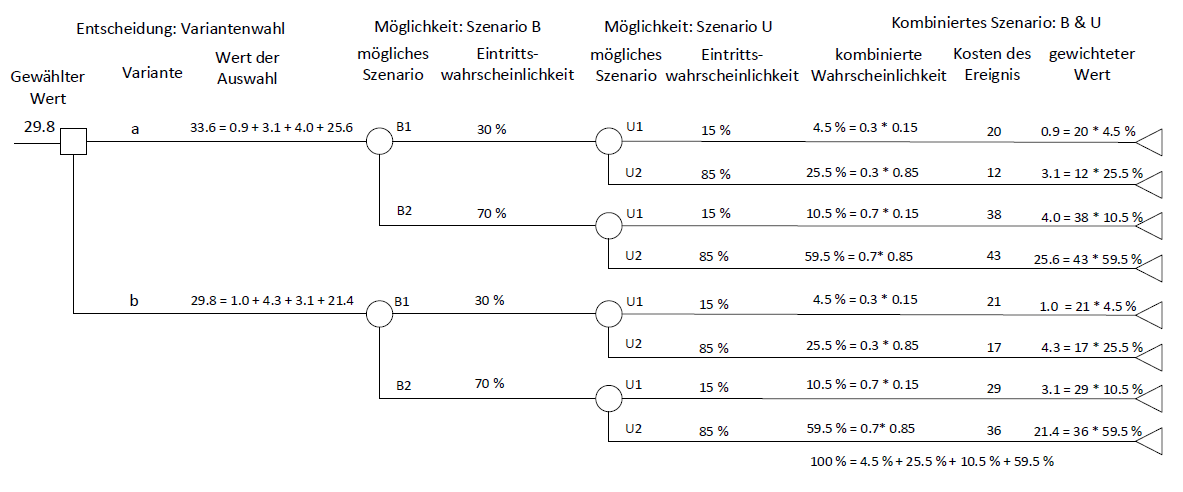
\includegraphics[width=\textwidth]{figures/f-02-02-EntscheidungsbaumBSP}
	\caption[Beispiel Entscheidungsbaum]{Beispiel eines Entscheidungsbaumes}
	\label{img:EntscheidungBSP}
\end{figure}

Die Abbildung \ref{img:EntscheidungBSP} zeigt ein fiktives Beispiel eines Entscheidungsbaumes im Rahmen einer Variantenwahl. Gesucht wird die Variante, welche die geringsten zu erwartenden Kosten und somit das kleinste Risiko generiert. Die Berechnung der Kosten erfolgt in diesem Beispiel von rechts nach links, wobei der zeitliche Verlauf der Entscheidungssituation von links nach rechts dargestellt wird. 

\section{Sensitivitätsanalyse}
\label{sec:Sensitivität}

Ein wichtiger Bestandteil der Kosten-Nutzen Analyse ist, mithilfe einer Sensitivitätsanalyse zu untersuchen, wie stark ein Ergebnis von den getroffenen Annahmen abhängt und wie robust das Ergebnis auf eine Variation der Parameter reagiert. \\
Die Sensitivitätsanalyse kann sowohl mit den Nebenbedingungen als auch mit der Zielfunktion durchgeführt werden. In beiden Fällen wird untersucht, was bei einer Veränderung der ursprünglichen Annahmen passiert und in welchem Rahmen die Parameter verändert werden können, ohne dass sich das ursprüngliche Ergebnis verändert.  (\cite{Adey2019})

\pagebreak
 
\section{Real Option Methodology}
\label{sec:RealOption}

Die \textit{Real Option Methodology} ist ein Vorgehen, um die optimale Variante einer Intervention unter Berücksichtigung von unsicheren zukünftigen Gegebenheiten zu bestimmen. Sie ermöglicht es, Varianten einer Infrastruktur Intervention zu erarbeiten, die auf zukünftige veränderliche Rahmenbedingungen ausgerichtet sind. So kann das Einbeziehen von flexiblen Designs im Prozess einer Infrastrukturintervention zusätzliche Vorteile generieren sowie zukünftige Risiken beseitigen. (\cite{Neufville2011})

Infrastrukturen sollten über einen längeren Zeitraum hinweg ihre Serviceleistung auf einem angemessenen Niveau erbringen können. Dies setzt voraus, dass sich die Infrastruktur an veränderliche Bedingungen anpassen und die Bedürfnisse der Interessensgruppen über einen längeren Zeitraum erfüllen kann. 
Mit dieser Methodik kann unter Berücksichtigung von unsicheren Variablen, wie zum Beispiel der Veränderung der Anzahl Nutzer oder der Baukosten, ermittelt werden, welches Design den Netto-Nutzen des Investors maximiert. (\cite{Esders2015})




% ===========================================================================
% EOF
%

%%% Local Variables:
%%% mode: latex
%%% TeX-master: "../main"
%%% End:
